% ----- Presentation -----

\subsection{Presentation}

    A \textbf{heuristic algorithm} is a type of algorithm that uses rules of thumb to try to find an approximate solution to a problem, rather than an exact one. Heuristic algorithms are often used when it is not possible to find an ideal solution to a problem, or when a perfect solution would be too time-consuming to compute. They are also used when an approximate solution is good enough, or when finding a flawless solution is not the primary goal. Heuristic algorithms are commonly used in artificial intelligence, computer science, and other fields. They are often used to solve optimization problems, search problems, and other types of problems where an exact solution is not necessary or practical.
    \\ \\
    A \textbf{constructive heuristic} algorithm is a type of heuristic algorithm that is used to find a solution to a problem by building it incrementally. Constructive heuristics start with a partial solution and gradually add to it until a complete solution is found. They are commonly used to solve optimization problems, where the goal is to find the optimal solution, or the solution that is the best among all possible solutions.
    \\ \\
    As we said, the use of the constructive heuristic in solving the MEWC start with a partial solution and build it until a complete solution is found. To do this, the latter will be subject to a number of criteria. 

    \begin{enumerate}
        \item Add The First Vertex to solution.
        \item Seek for his most weighted neighbors. And add it to solution if it's a neighbor of all vertices in solution(to be sure to hold a clique in the final result). Store the weight of the edge between every members of the solution and the new vertex.
        \item Repeat the step 2 until no vertices is available to add
    \end{enumerate}

    We will then have for solution a maximum clique with his weight. 
    \\ \\
    In these choices of criteria, we can notice one that is quite important. The one to choose the First Vertex. Indeed, it is this one which will define the quality of our solution. Taking it randomly would be useless and counter productive for the sake of solving MEWC. As it was important, we thought about how to choose it and 2 answers appeared to us and we have a debate on the subject because we could not reach a consensus on it. We hesitated between these two solutions:

    \begin{itemize}
        \item The first idea was to take the highest degree vertex of the graph given as input. 
        \begin{itemize}
            \item One reason to choose the highest degree vertex as the first vertex in the solution is that it may be more likely to be part of a maximum edge weight clique(because it's the case where it's the most likely to have the biggest clique who could be the MEWC). This is because it will allow more edges to be added to the solution, which can increase the overall sum of edge weights in the clique.
            \item Another reason is that it may be more likely to be connected to other high degree vertices. This means that by adding the highest degree vertex to the clique first, we may be able to include other high degree vertices in the clique as well, which can further increase the overall sum of edge weights.
        \end{itemize}
        \item The second one was to take the vertex with the highest sum of weights of the edges.
        \begin{itemize}
            \item One reason to choose the vertex with the highest edge weight as the first vertex in the clique is that it may be more likely to be part of a maximum edge weight clique. This is because adding a vertex with a high edge weight to the clique will contribute more to the overall sum of edge weights in the clique, which is what we are trying to maximize.
            \item Another reason is that we can potentially reduce the search space for the rest of the algorithm. This is because we know that any clique we find must include this vertex, which means that we can eliminate any vertices that are not connected to it as potential members of the clique. This can help to make the algorithm more efficient by reducing the number of vertices that we need to consider.
        \end{itemize}
    \end{itemize}
    
    We will illustrate these explanations with figure 11 and 12 which shows the advantages of each over the other.
    \\ \\
    \begin{minipage}{\linewidth}
        \begin{minipage}{0.5\textwidth}
            \begin{figure}[H]
                \centering
                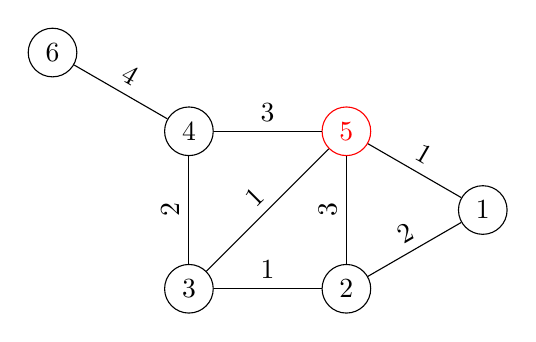
\begin{tikzpicture}[node distance=2cm]
                    \node[circle, draw] (1) {1};
                    \node[circle, draw] (2) at ([shift=(210:2)] 1) {2};
                    \node[circle, draw] (3) [left of=2] {3};
                    \node[circle, draw] (4) [above of=3] {4};
                    \node[circle, draw, red] (5) [above of=2] {5};
                    \node[circle, draw] (6) at ([shift=(150:2)] 4) {6};
    
                    \draw  (1) -- (2) node[midway, above, sloped] {2};
                    \draw (1) -- (5) node[midway, above, sloped] {1};
                    \draw (2) -- (3) node[midway, above, sloped] {1};
                    \draw (2) -- (5) node[midway, above, sloped] {3};
                    \draw (3) -- (4) node[midway, above, sloped] {2};
                    \draw (4) -- (5) node[midway, above, sloped] {3};
                    \draw (4) -- (6) node[midway, above, sloped] {4};
                    \draw (5) -- (3) node[midway, above, sloped] {1};
                \end{tikzpicture}
                \caption{Graph illustration for the highest degree vertex}
                \label{fig:vertex-highest-degree}
            \end{figure}
        \end{minipage}
        \begin{minipage}{0.5\textwidth}
            \begin{figure}[H]
                \centering
                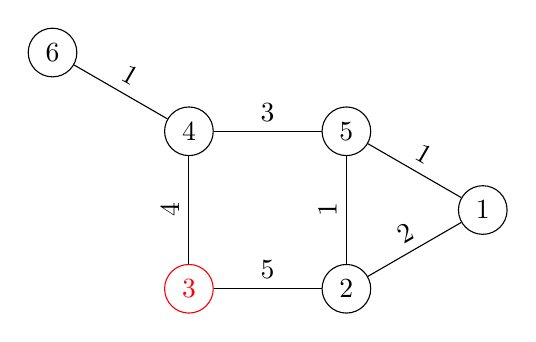
\begin{tikzpicture}[node distance=2cm]
                    \node[circle, draw] (1) {1};
                    \node[circle, draw] (2) at ([shift=(210:2)] 1) {2};
                    \node[circle, draw, red] (3) [left of=2] {3};
                    \node[circle, draw] (4) [above of=3] {4};
                    \node[circle, draw] (5) [above of=2] {5};
                    \node[circle, draw] (6) at ([shift=(150:2)] 4) {6};
    
                    \draw  (1) -- (2) node[midway, above, sloped] {2};
                    \draw (1) -- (5) node[midway, above, sloped] {1};
                    \draw (2) -- (3) node[midway, above, sloped] {5};
                    \draw (2) -- (5) node[midway, above, sloped] {1};
                    \draw (3) -- (4) node[midway, above, sloped] {4};
                    \draw (4) -- (5) node[midway, above, sloped] {3};
                    \draw (4) -- (6) node[midway, above, sloped] {1};
                \end{tikzpicture}
                \caption{Graph illustration for the vertex with the highest sum of weights of the edges}
                \label{fig:vertex-best-sum-weight-edge}
            \end{figure}
        \end{minipage}
    \end{minipage}

    \vspace{1\baselineskip}

    We implemented both ideas and performed tests on a number of graph to see which was the most consistent and we concluded that it was the vertex with the highest sum of weights of the edges. Moreover, in most graphs (at least the randomly generated ones), we had, in general, a rather homogeneous weights of edges which worked better with this one.
    \\ \\
    Constructive heuristic can be contrasted with other types of heuristics, such as local search heuristics, which try to find a solution by making small changes to an existing solution, or random heuristics, which generate solutions randomly and then choose the best one. Constructive heuristics are often used when it is important to find a solution that is complete and comprehensive, rather than just a local improvement.
    \\ \\
    Examples of some famous problems that are solved using constructive heuristics are the flow shop scheduling, the vehicle routing problem and the open shop problem.
    
    